\section*{2 - Including figures and results}
Here are some examples of including figures in your latex document...

A simple centred figure with a label and caption.
\begin{figure}[H]
\centering
\caption{Time course of membrane potential in simulation}
\label{fig:q1a}
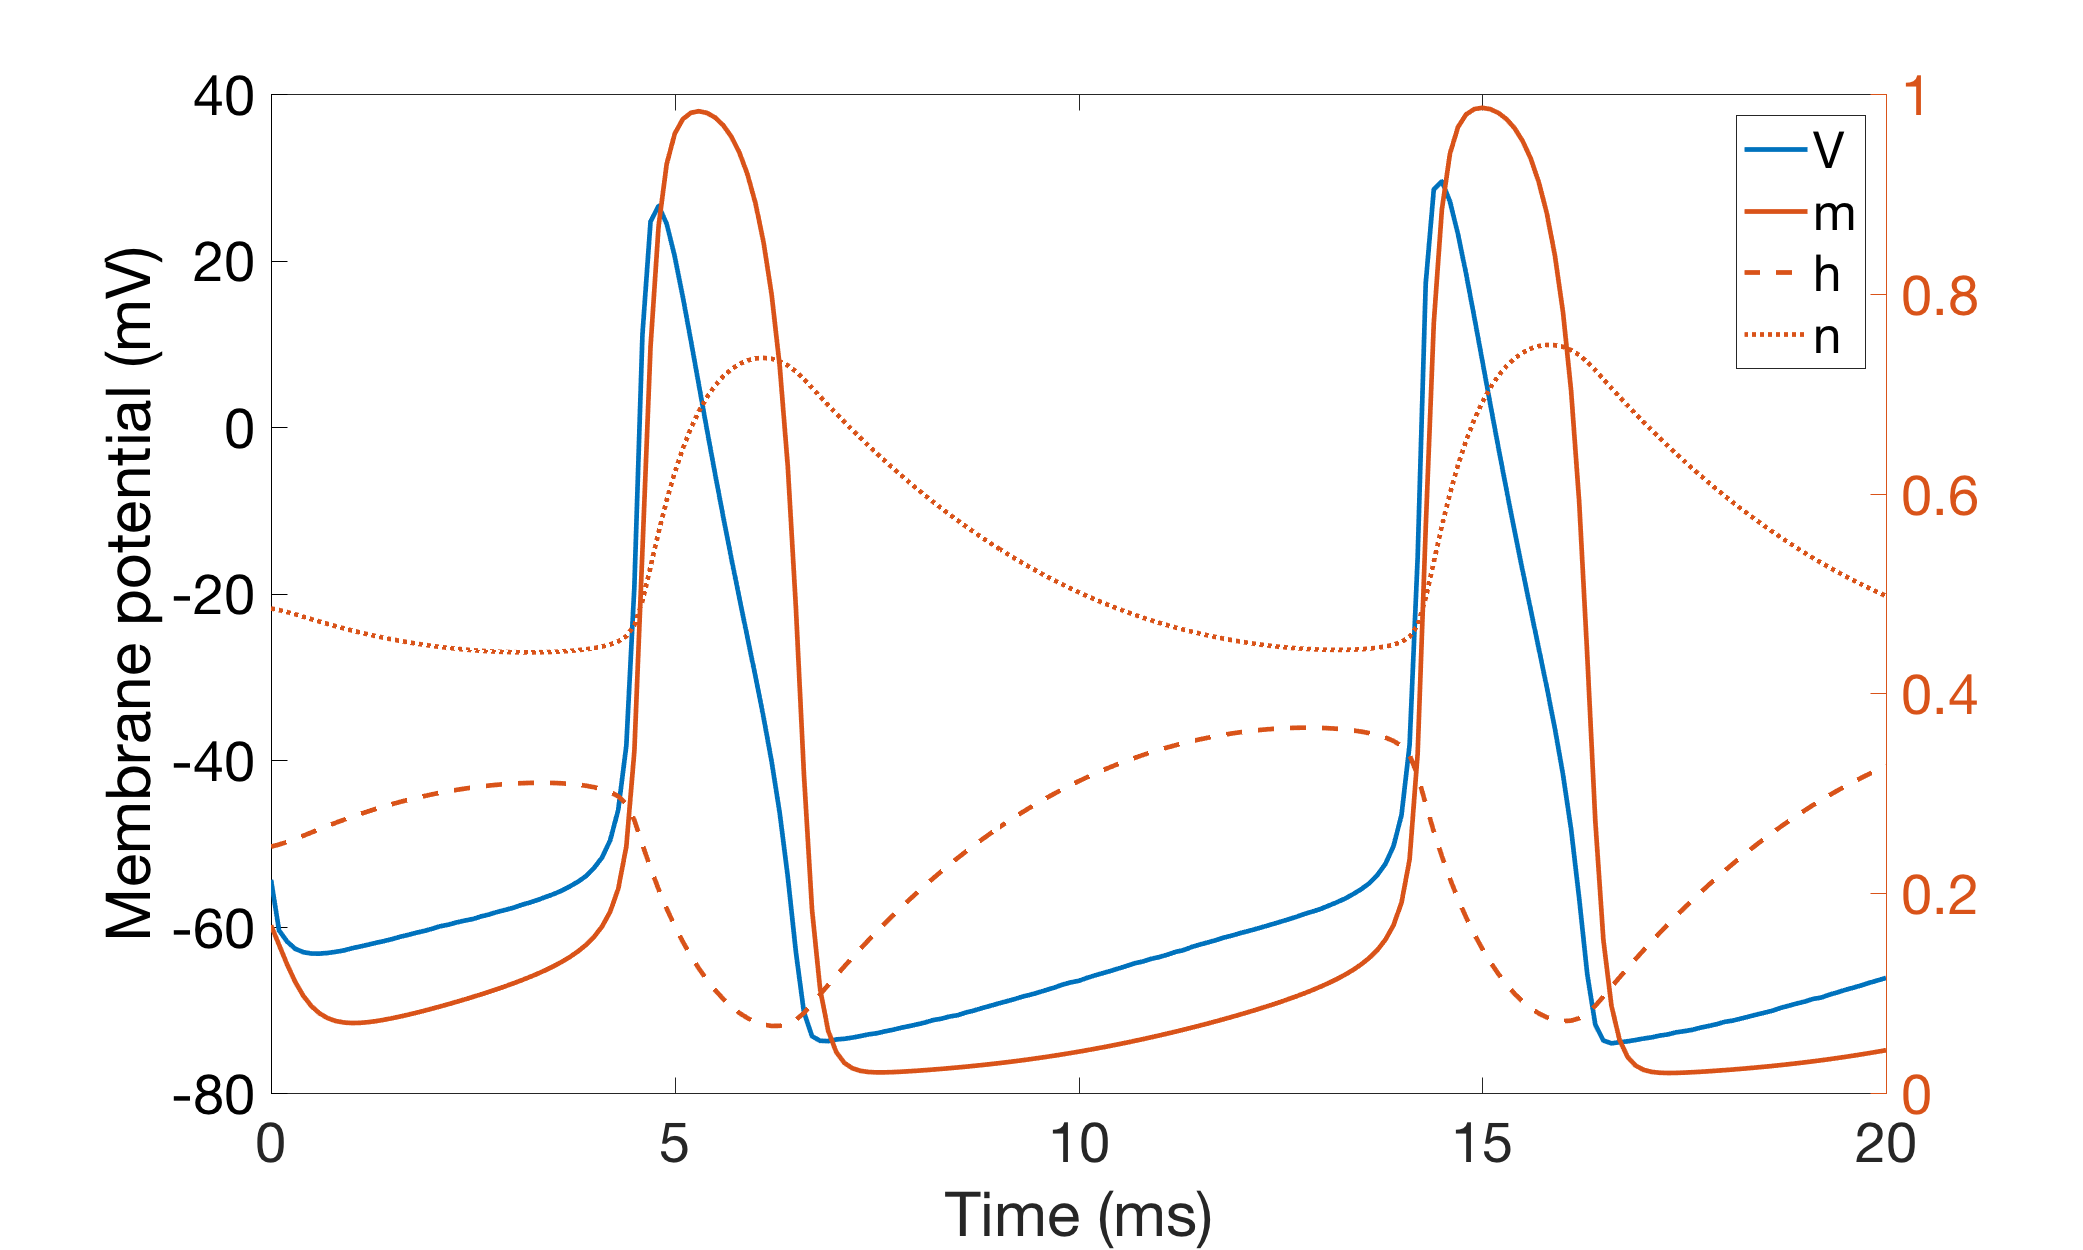
\includegraphics[scale=0.3]{exp-results.png}    
\end{figure}

Two figures side by side, centered.
\begin{figure}[H]
\centering
\begin{subfigure}[c]{0.4\textwidth}
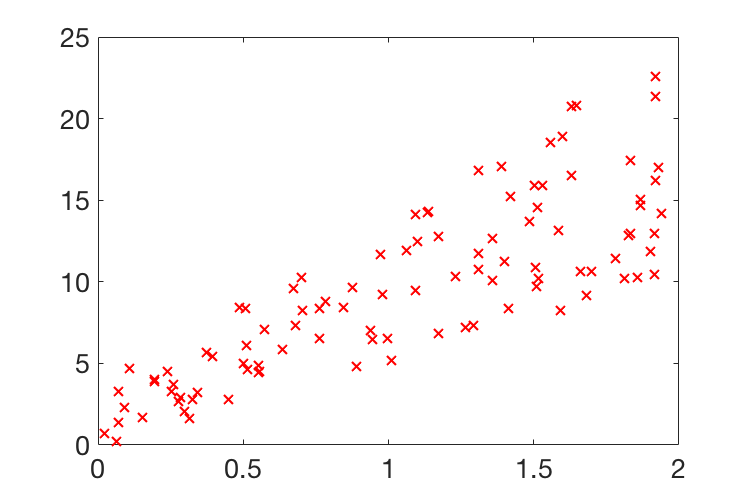
\includegraphics[width=0.9\linewidth]{fig1}
\caption{first caption}
\label{fig:subim1}
\end{subfigure}
\begin{subfigure}[c]{0.4\textwidth}
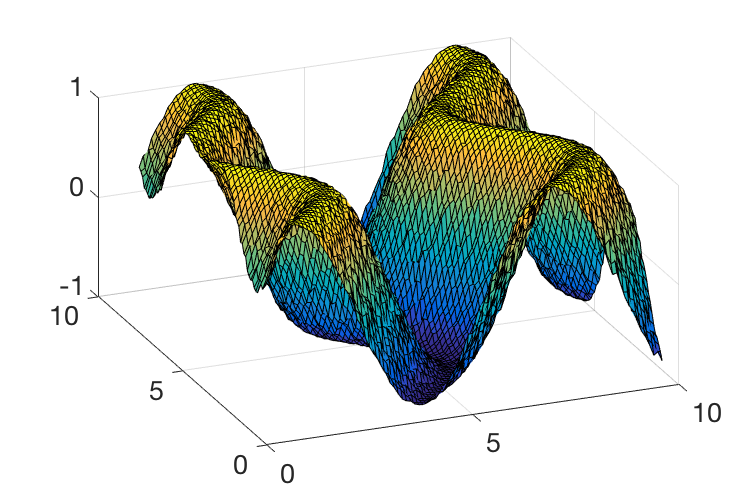
\includegraphics[width=0.9\linewidth]{fig2}
\caption{second caption}
\label{fig:subim2}
\end{subfigure}
 
\caption{Caption for this figure with two images}
\label{fig:image2}
\end{figure}

A simple table of results.
\begin{center}
\begin{tabular}{ |c|c|c|c|c| } 
 \hline
 Experiment & 1 & 2 &
3 & 4 \\ 
 \hline
 Metric 1 &
 1.2 & 3.4 & 5.4 & 4.2 \\
 Metric 2 &
 86.3\% & 24.6\% & 42.4\% & 59.1\% \\ 
 \hline
\end{tabular}
\end{center}
